\documentclass{article}

\usepackage{arxiv}

%%% Columns
\usepackage{multicol}

%%% Polices et langue
\usepackage[hyphens]{url}         % Pour citer les adresses web
\usepackage{hyperref}             % Citations plus complètes
\usepackage[T1]{fontenc}          % Encodage des accents
\usepackage[utf8]{inputenc}       % Lui aussi

%%% Couleurs et modification sur l'écriture
\usepackage[svgnames]{xcolor}     % De la couleur
\usepackage{cancel}               % Pour les traits
% \usepackage[margin=2cm]{geometry} % Gérer correctement la taille
\usepackage{enumitem}

%%% Symboles mathématiques
\usepackage{amsmath}              % La base pour les maths
\usepackage{mathrsfs}             % Quelques symboles supplémentaires
\usepackage{amssymb}              % encore des symboles.
\usepackage{amsfonts}             % Des fonts, eg pour \mathbb.

%%% Pour les dessins, les graphiques, ...
\usepackage{stackengine}
\usepackage{float}
\usepackage{graphicx}             % inclusion des graphiques
\usepackage{caption}
\usepackage{subcaption}
\usepackage{wrapfig}              % Dessins dans le texte
\usepackage{array}                % Pour avoir des colonnes personnalisées
\newcolumntype{P}[1]{>{\centering\arraybackslash}p{#1}} % Colonne centrée
\usepackage{makecell}             % Allow for intricated tables

%%% Pour représenter les algorithmes
\usepackage[noend, ruled, french, onelanguage]{algorithm2e}

%%% Special commands

% Uncomment to remove the header
\pagestyle{plain}

% Uncomment to override  the `A preprint' in the header
\renewcommand{\headeright}{}
\renewcommand{\undertitle}{}
% \renewcommand{\shorttitle}{\textit{arXiv} Template}

% Les guillemets \ofg{par exemple}
\newcommand{\ofg}[1]{\og{}#1\fg{}}
% Des parenthèses, crochets et accolades qui s'adaptent automatiquement à
% la taille de ce qu'il y a dedans
\newcommand{\pa}[1]{\left(#1\right)}
\newcommand{\pac}[1]{\left[#1\right]}
\newcommand{\paa}[1]{\left\{#1\right\}}
% Pour faire des indices en mode texte
\newcommand{\e}[1]{_{\text{#1}}}
% Pour avoir une couleur uniquement sur les traits
\newcommand{\Cancel}[2][black]{{\color{#1}\cancel{\color{black}#2}}}

% Customized bibliography
\let\OLDthebibliography\thebibliography
\renewcommand\thebibliography[1]{
  \OLDthebibliography{#1}
  \setlength{\parskip}{0pt}
  \setlength{\itemsep}{0pt plus 0.3ex}
}

% For having figures in the two-column environment
\newenvironment{Figure}
  {\par\medskip\noindent\minipage{\linewidth}}
  {\endminipage\par\medskip}

%%% Title

% Mettez votre titre et votre nom ci-après
\title{Cover Type Prediction}
\author{
  \textbf{Sébastien Meyer} \\
  École polytechnique, France \\
  \texttt{sebastien.meyer@polytechnique.edu}
}
% À décommenter si vous ne voulez pas que la date apparaisse explicitement
\date{}

%%% The document itself

\begin{document}

\maketitle

\begin{multicols}{2}

This report details the different approaches and strategies that I have developed in order
to get the best possible score I could on the cover type data set. We were given a
dataset made up of a
gathering of different numerical and qualitative features describing $30 \times 30$ meter
forest cells. The main task was to predict the cover type of each of these cells. We had
a training set and we were asked to submit a prediction containing a cover type associated
to each
cell, some of them being taken from the training set and others being brand-new data.

Despite the fact that this dataset is well-known since its donation to the UCI in
1998\footnote{\url{https://archive.ics.uci.edu/ml/datasets/covertype}},
and after past Kaggle
competitions\footnote{\url{https://www.kaggle.com/c/forest-cover-type-prediction}}, it has
been a really challenging project for me. In order
to best describe how I tackled this problem, my report will follow my advances. Firstly, I
will remind the reader with a brief description of the task and the data. Then, I will go on
with my first attempts. Since my first tries were not satisfactory,
I took inspiration from past Kaggle competitions - both on this dataset and others - to get
new ideas. In the 
\textbf{Appendix}, I gathered my models with some details on the
pipeline, as well as a description of the engineered features.

\section{The dataset}

The dataset is made up of 15120 training points and 581012 test points. It appears that the
training
points are also part of the test set, which is interesting and should ensure a certain
accuracy of any model. However, we can already note that the test set is much larger than
the training set and that it might contain different distributions of data. Therefore, we
must be prepared to face overfitting. Our task is a classification task, corresponding to
the \textit{Cover\_Type} feature which
ranges between 1 and 7. The training set is quite imbalanced, as each class does not account for
2160 of the 15120 samples (see \textbf{Figure \ref{fig:labelrepart}}).

\begin{Figure}
    \centering
    \captionsetup{type=figure}
    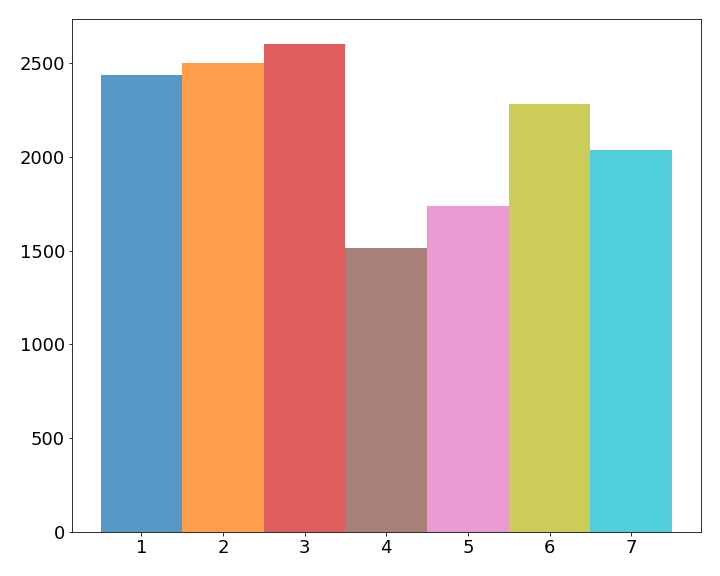
\includegraphics[width=0.75\linewidth]{figures/label_repart.png}
    \captionof{figure}{Repartition of the training labels.}
    \label{fig:labelrepart}
\end{Figure}

Also, there are 54
available features. 40 of them correspond to \textit{Soil\_TypeX} with \textit{X} ranging
between 1 and 40. Each data point is assigned with one and only one \textit{Soil\_TypeX}
feature, which gets the value 1. Same goes for 4 other features which are
\textit{Wilderness\_AreaY} with \textit{Y} ranging between 1 and 4. Finally, the ten last
features are briefly summarized in \textbf{Table \ref{tab:featsum}}. Only
\textit{Vertical\_Distance\_To\_Hydrology} has negative values for some of the data points,
while all the other features are nonnegative. The \textit{Cover\_TypeX} and
\textit{Wilderness\_AreaY} features could have a huge impact on our predictions, because
of them being uniquely assigned to the data points. Also, they are highly correlated
with our target feature. In \textbf{Figure \ref{fig:basecorr}}, we show the four features
that are the most correlated with our target feature. Overall, there is no correlation
over 0.6 between two features, which does not lead us to exclude any feature here.
However, the \textit{Soil\_TypeX}
features are differently distributed, with a number of associated data points ranging
from zero for \textit{Soil\_Type15} to thousands for some soil types.

\begin{center}
\captionsetup{type=tabular}
\begin{tabular}{|c|cccc|}
    \hline
    Feature & Mean & Std & Min. & Max. \\
    \hline
    Elevation & 2,749 & 419 & 1,877 & 3,850 \\
    Aspect & 156 & 110 & 0 & 360 \\
    Slope & 16.56 & 8.53 & 0 & 50 \\
    Horz Hyd & 228 & 209 & 0 & 1,376 \\
    Vert Hyd & 51.31 & 61.52 & -135 & 570 \\
    Horz Road & 1,718 & 1,330 & 0 & 6,803 \\
    Horz Fire & 1,527 & 1,117 & 0 & 7,095 \\
    Hill 9AM & 213 & 30.64 & 52 & 254 \\
    Hill Noon & 219 & 22.80 & 99 & 254 \\
    Hill 3PM & 134 & 46.07 & 0 & 251 \\
    \hline
\end{tabular}
\captionof{table}{Description of numerical features.}
\label{tab:featsum}
\end{center}

\begin{Figure}
    \centering
    \captionsetup{type=figure}
    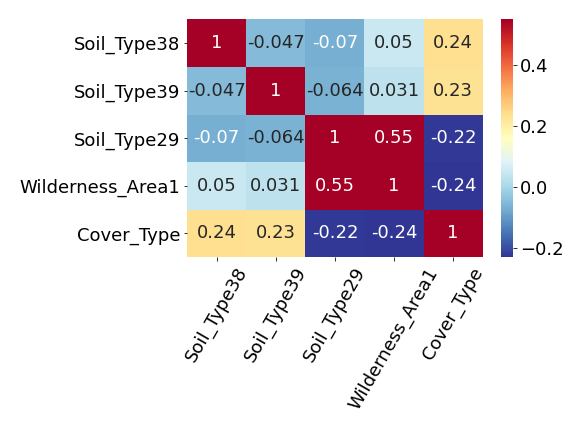
\includegraphics[width=0.85\linewidth]{figures/basecorr.png}
    \captionof{figure}{Simplified correlation matrix.}
    \label{fig:basecorr}
\end{Figure}

\section{First attempts}

After my first data exploration, I decided to try out some basic
models that are widely used for multiclass classification. I did not
do much feature engineering, apart from removing the \textit{Cover\_Type15}
feature which is assigned to no data point. Moreover, I decided to
merge the binary features into one feature, for instance
\textit{Soil\_Type} with values ranging from 1 to 40 assigned to each
data point and \textit{Wilderness\_Area} ranging from 1 to 4. Rapidly,
I understood that this would not help building more accurate predictions.
Indeed, when we do merge several binary features into only one, we
induce a fictive ordering between values. Let $X$ be a feature gathering
binary features and thus having values from 1 to $p$. When splitting
at a specific node,
a decision tree can make a decision based on $X > a$ or $X \leq a$.
We see that such decision implies that values between 1 and $a$ have
a relationship, which might not be the case. Therefore, we cannot
expect accurate predictions by doing so.

\subsection{Cross-validated gridsearch}

I implemented an automated gridsearch pipeline
using \textit{optuna} package to select the parameters of any model
I decided to use. \textit{Optuna}\cite{optuna} takes ranges of values for
model parameters as entry, and performs an optimization to find the best
parameters according to the cross-validation score. The cross-validation
was 5 folds large, with accuracy as target. Typically, I would run a
gridsearch for 15 to 50 trials, depending on the complexity of the model
and the size of the dataset.

\subsection{RandomForestClassifier and LightGBM}

The first two models that I used were RandomForestClassifier and
LightGBM\cite{lightgbm}
from \textit{scikit-learn}\cite{sklearn} API.
These models are widely used in the case of classifications with more
than two possible labels. For instance, RandomForestClassifier relies on
the averaging of several base decision trees. These decision
trees are built in a top-bottom fashion. Each split builds two nodes or
regions $R$ and $\bar{R}$. Let us denote by $p^{R}_k$ and $p^{\bar{R}}_k$
the proportions of samples from class $k$ falling respectively in regions
$R$ and $\bar{R}$. Split is made by minimizing a criterion, the most used
criterion being Gini index defined as:

\begin{center}
  $$
  C(R, \bar{R}) = \sum \limits_{k} p^R_k (1 - p^R_k) +
  \sum \limits_{k} p^{\bar{R}}_k (1 - p^{\bar{R}}_k)
  $$
\end{center}

\noindent which is the sum of Gini impurities in both $R$ and $\bar{R}$.
Other criterions can be used and have been tried during gridsearch, namely entropy
criterion, however Gini index yields best results in almost all runs. On the other
hand, LightGBM is based on Boosting rather than Bagging. Although LightGBM is based
on the same principle as other Boosting models, that is, updating a model by
successively assigning weights to wrongly classified data points, it is designed to
be much more faster on large datasets than its counterparts.

\begin{Figure}
  \centering
  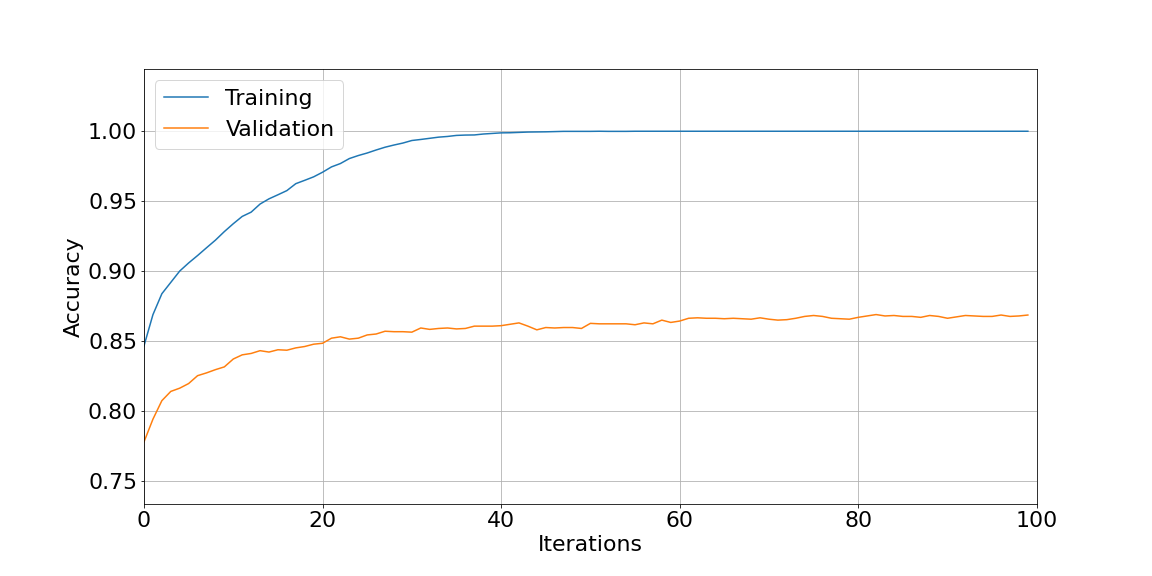
\includegraphics[width=\linewidth]{figures/lgbmeval.png}
  \captionsetup{type=figure}
  \captionof{figure}{Learning curves for LightGBM.}
  \label{fig:lgbmeval}
\end{Figure}

A basic
gridsearch for RandomForestClassifier
lead to an accuracy of 0.7613, and a basic gridsearch for LightGBM lead to an accuracy of 0.78374. These scores
were relatively good, considering that I did not started feature engineering
and that my models were rather simple. However, tweaking these models did not bring much
improvement. I had to start engineering new features.

\section{Taking inspiration from past competitions}

\subsection{New features}

As for most of the Kaggle competitions, feature engineering is mandatory for
getting better scores. Looking at the available features, I computed some new
features: \textit{Distance\_To\_Hydrology} is built as the square root of
the sum of \textit{Horizontal\_Distance\_To\_Hydrology}² and
\textit{Vertical\_Distance\_To\_Hydrology}²; \textit{Ratio\_Distance\_To\_Hydrology}
is built as \textit{Vertical\_Distance\_To\_Hydrology} over
\textit{Horizontal\_Distance\_To\_Hydrology} (when dividing by zero, value is
replaced by the median of finite values);
\textit{Horizontal\_Distance\_To\_Point\_Log} is built as
$\log(1+\text{\textit{Horizontal\_Distance\_To\_Point}})$ for
\textit{Point} being \textit{Hydrology}, \textit{Roadways} and \textit{Fire\_Points};
\textit{Aspect\_times\_Hillshade\_3pm} is built as the product of the features
(relation derived from their closeness in a simple hierarchical clustering);
all possible polynomial combination of some chosen numerical features.

Then, the base and engineered features were still not enough. After looking
at some discussions on past Kaggle competitions, I started another
data exploration. Simple statistics such as \textit{Max}, \textit{Min} or 
\textit{Mean} can be added
to the features. On top of that, new distances can be approximated from those
in our possession. Indeed, the horizontal distance between hydrology and roadways is
somewhere between \textit{Horizontal\_Distance\_To\_Hydrology} $-$
\textit{Horizontal\_Distance\_To\_Roadways} in absolute value and
\textit{Horizontal\_Distance\_To\_Hydrology} $+$
\textit{Horizontal\_Distance\_To\_Roadways}. Thus, I added all the absolute
differences and sums of these distances, as well as the mean distance to
all three points of interest.

\begin{Figure}
  \centering
  \captionsetup{type=figure}
  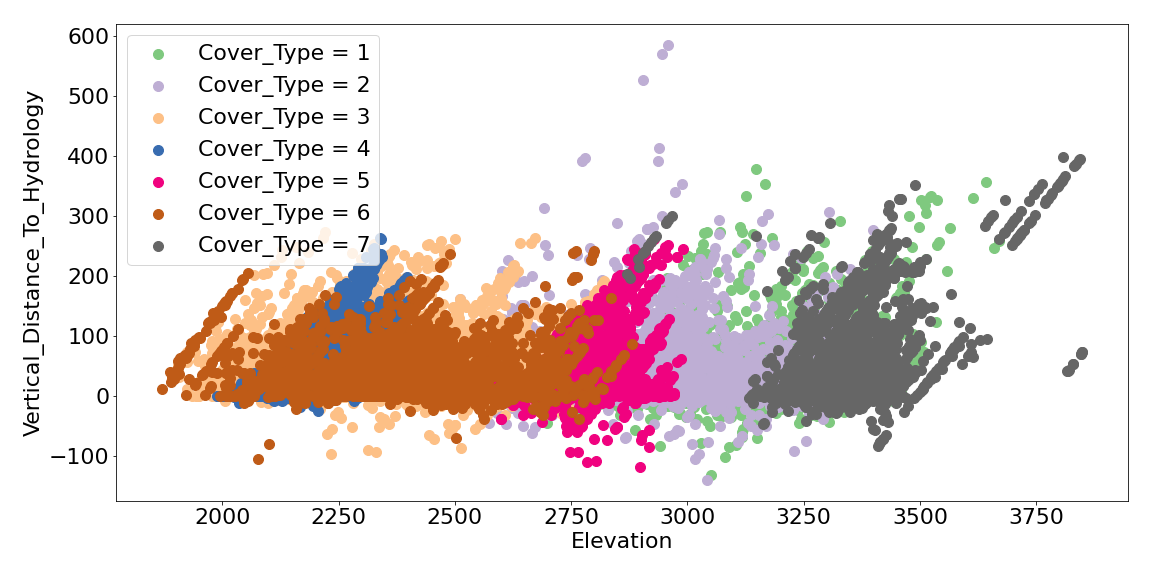
\includegraphics[width=0.85\linewidth]{figures/elevverthyd.png}
  \captionof{figure}{Relationship between \textit{Elevation} and
                     \textit{Vertical\_Distance\_To\_Hydrology}.}
  \label{fig:elevverthyd}
\end{Figure}

\begin{Figure}
  \centering
  \captionsetup{type=figure}
  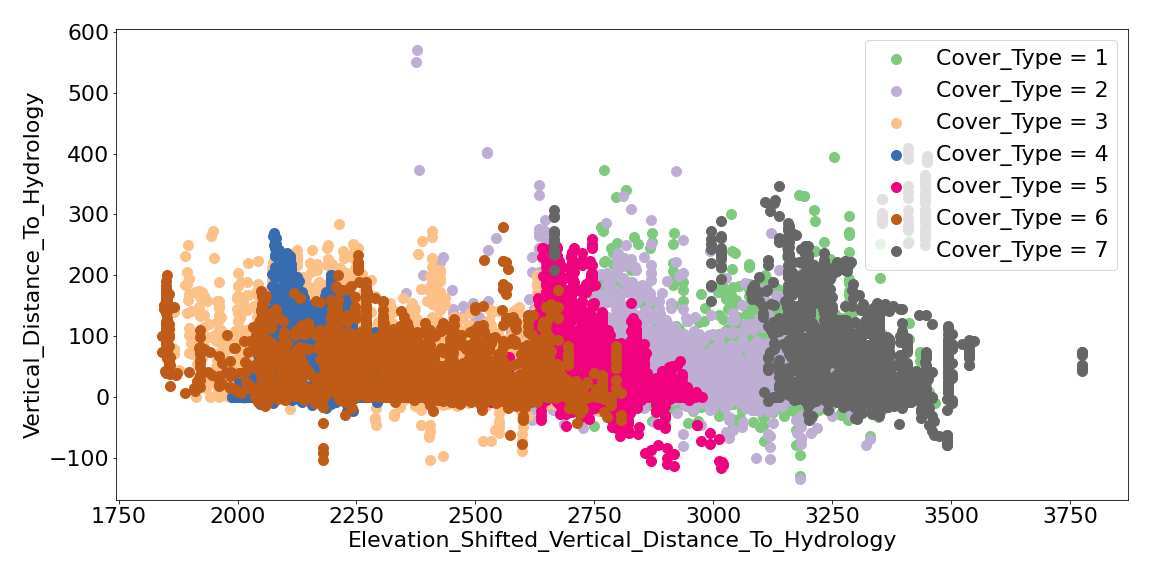
\includegraphics[width=0.85\linewidth]{figures/elevshiftverthyd.png}
  \captionof{figure}{Relationship between \textit{Elevation} and
                     \textit{Elevation\_\\Shifted\_Vertical\_Distance\_To\_Hydrology}.}
  \label{fig:elevshiftverthyd}
\end{Figure}

One of the most important features can be easily derived
from the available data. As shown \textbf{Figure \ref{fig:elevverthyd}}, the relationship
between \textit{Elevation} and \textit{Vertical\_Distance\_To\_Hydrology} is
affine. As a result, simple borders between cover types can be derived by
a linear model such as a Random Forest if we manage to align a new feature
with \textit{Elevation}. As shown \textbf{Figure \ref{fig:elevshiftverthyd}}, it
is relatively easy to compute such a feature. Same can be done with
\textit{Horizontal\_Distance\_To\_Hydrology} and
\textit{Horizontal\_Distance\_To\_Roadways}. These new features are appended
with the \textit{Shifted} mark. An example of resulting repartition of
training labels wrt a new feature is shown \textbf{Figure \ref{fig:elevshiftverthydrep}}.

\begin{Figure}
  \centering
  \captionsetup{type=figure}
  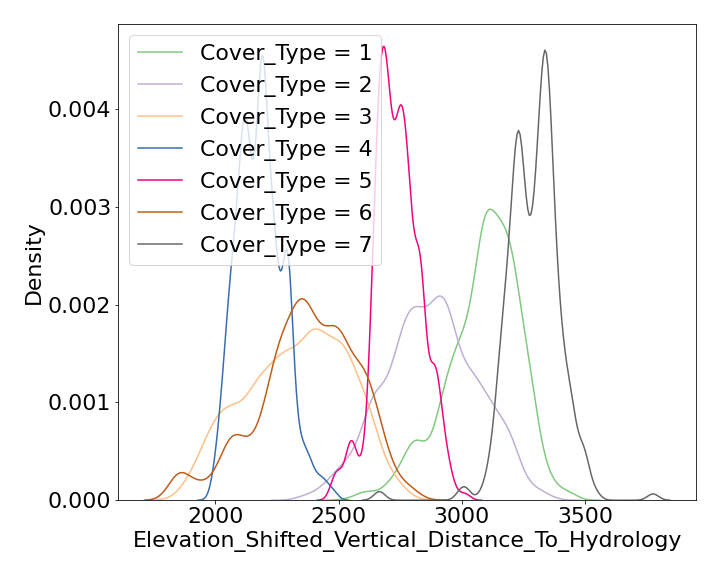
\includegraphics[width=0.75\linewidth]{figures/elevshiftverthydrep.png}
  \captionof{figure}{Repartition of training labels wrt
                  \textit{Elevation\_Shifted\_Vertical\_Distance\_To\_Hydrology}.}
  \label{fig:elevshiftverthydrep}
\end{Figure}

\subsection{ExtraTreesClassifier and OneVsRestClassifier}

Thanks to these new features, RandomForestClassifier was able to outperform
LightGBM and its accuracy approached 0.87 during cross-validation.
Nevertheless, another great 
improvement
for this dataset stems from the use of ExtraTreesClassifier. This classifier is
based on trees that differ from usual decision trees in two points:

\begin{enumerate}[wide, labelindent=5pt, itemsep=0pt, topsep=0pt]
  \item Bootstrapping is disabled by default for ExtraTreesClassifier
  \item Splits are chosen among randomly drawn cuts given a subset of features
\end{enumerate}

In some cases, such extremely randomized decisions can reduce overfitting,
as it appears to be the case for this dataset. Indeed, the absolute difference in
accuracy between training and validation was much smaller with ExtraTreesClassifier.
My first trial with these
new features and ExtraTreesClassifier obtained an accuracy of 0.82237. Going further,
I started adding more features and manually tried to find the best subset of
features. Therefore, I decided to compute polynomial features from a different
subset of base and engineered features. Also, I used a OneVsRestClassifier from
\textit{scikit-learn}, which focuses on fitting one classifier per class in
a "one-vs-all" fashion. All these slight improvements allow me to reach an accuracy of 0.82622.

\subsection{Failed attempts}

Once feature engineering was done, features would easily 
exceed 100 when counting 
polynomial features. I thought that such a number of features could lead to 
overfitting or that we could lose information due to correlation. In order 
to prevent this to happen, I tried two methods. First, I removed features that 
were too correlated (one per pair) with a fixed threshold. Second, 
I also tried to remove the features with a high variance inflation factor. 
Variance inflation factor is defined as $\text{VIF}_i = 1/(1 - R_i^2)$,
where $R_i^2$ is the R-squared value of a linear regression of feature 
$i$. This factor asseses the ability to estimate a feature thanks to the 
others and thus their correlation. However, removing features using these 
techniques always lead me to poorer accuracy. In addition, I 
ran PCA several times but the same problem occured.
\textbf{Figure \ref{fig:pca}} shows the evolution of the cross-validation 
accuracy with ExtraTreesClassifier when PCA is applied. Features are typically 
those that I used in my last trials (see next section or \textbf{Appendix}).

\begin{Figure}
  \centering
  \captionsetup{type=figure}
  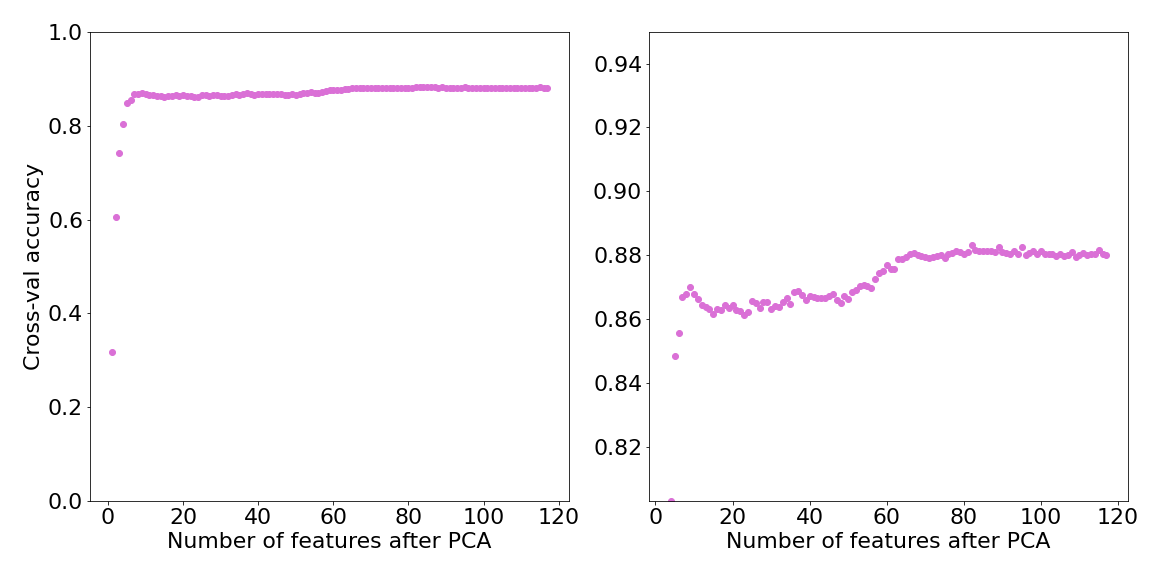
\includegraphics[width=0.85\linewidth]{figures/pca.png}
  \captionof{figure}{Evolution of cross-validation accuracy with number of PCA components.}
  \label{fig:pca}
\end{Figure}

Another model that I used is a simple feed-forward network. By tweaking 
some of the parameters, I was able to design a network with one hidden layer 
of approximately 50 neurons and sigmoid activation function, fitted with the 
RMSprop optimizer, which yielded 
relatively good results, nevertheless they were always below the scores 
of forest models. In my opinion, neural networks are more prone to overfitting 
in such context, moreover they often require lots of training data and features that 
we are in lack of in this data set.

\section{Last improvements}

\subsection{More features and data cleaning}

After that, I built some features and tried several combinations.They yielded only
small improvements. It can be noted that some of the features that
I have computed are the mean Hillshade index, binary features corresponding to
soil types families (there are 7 families plus a category for neither of them, as
detailed in the Data appendix) and soil types stonyness (either stony, rubly or
neither). An interesting observation that I made only during the last days of the
competition is about missing values for the \textit{Hillshade\_3pm} feature. As
shown \textbf{Figure \ref{fig:hill3pmbefore}}, there are too much zeros for it to be
natural.

\begin{Figure}
  \centering
  \captionsetup{type=figure}
  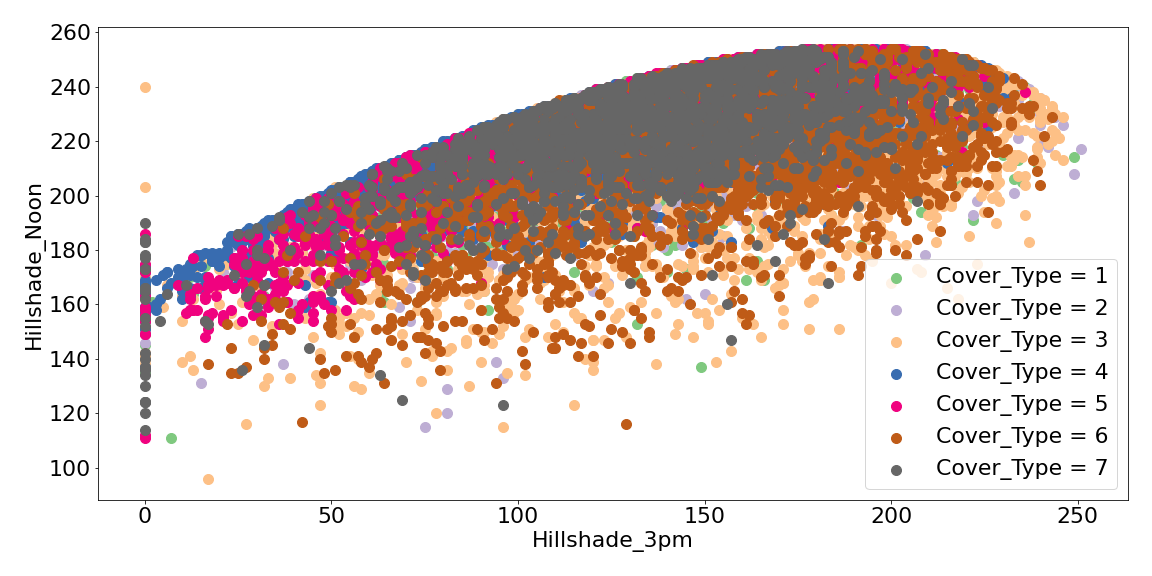
\includegraphics[width=0.85\linewidth]{figures/hill3pmbefore.png}
  \captionof{figure}{Training \textit{Hillshade\_3pm} values before estimation.}
  \label{fig:hill3pmbefore}
\end{Figure}

A simple technique to reduce the number of missing values is to estimate
them thanks to known values. Thus, I trained an ExtraTreesRegressor model using
all the other explanatory features of training data points where
\textit{Hillshade\_3pm} is positive.
Then, missing
values are
predicted both for training and test points. As shown
\textbf{Figure \ref{fig:hill3pmafter}}, we get a good estimation of at least
a part of the missing values.

\begin{Figure}
  \centering
  \captionsetup{type=figure}
  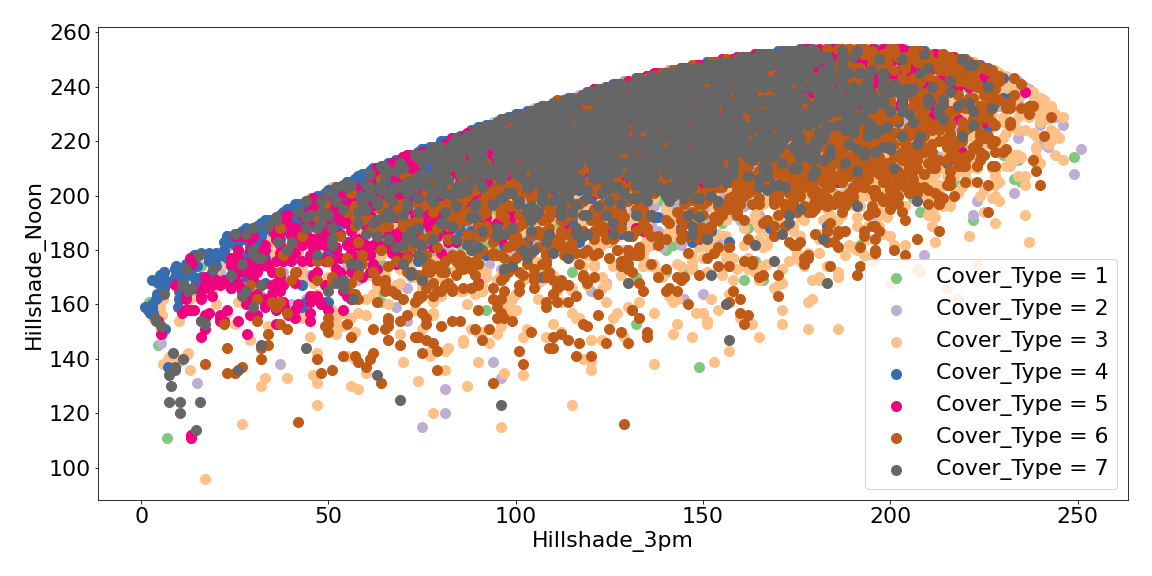
\includegraphics[width=0.85\linewidth]{figures/hill3pmafter.png}
  \captionof{figure}{Training \textit{Hillshade\_3pm} values after estimation.}
  \label{fig:hill3pmafter}
\end{Figure}

\subsection{Stacking}

Even though ExtraTreesClassifier appears to outperform other models, Boosting
models such as LightGBM and XGBoost\cite{xgboost} perform relatively well on
the dataset and
RandomForestClassifier yields similar results to Boosting. One of the methods
used to combine different models that can be good at predicting specific aspects
of the data is through Stacking. In the \textit{scikit-learn} API, several base
models are fitted
on the training dataset. Then, a final estimator - usually a LogisticRegression -
is fitted on base estimators predictions over training data with cross-validation
to avoid overfitting. A summary schema is shown \textbf{Figure \ref{fig:stacking}}.
In this model, I tried to combine different models such as
RandomForestClassifier, ExtraTreesClassifier and LightGBM. Adding XGBoost yielded
slight to no improvement.

\begin{Figure}
  \centering
  \captionsetup{type=figure}
  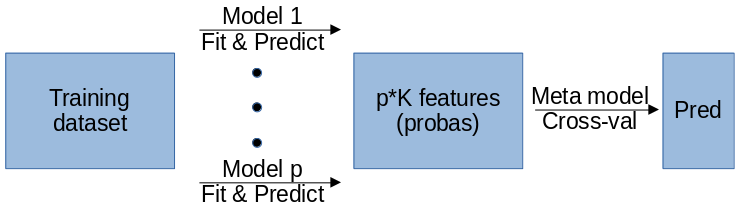
\includegraphics[width=0.75\linewidth]{figures/stacking_schema.png}
  \captionof{figure}{Stacking pipeline.}
  \label{fig:stacking}
\end{Figure}

Since Stacking uses several models, its training is much more longer than for
any base estimator. Therefore, running a gridsearch for the Stacking model would
be computationally too expensive for my computer. I decided to fix the parameters
of the base estimators using the best parameters of their own gridsearch.
Together with some more features, Stacking allowed me to reach an accuracy
of 0.83822.

\subsection{Resampling the training dataset}

One of the major issues that I observed in this challenge is that, there were
huge differences in accuracy between cross-validation and final score. Clearly,
one can expect a poorer accuracy between training and validation, mostly due to
overfitting. However, I observed a difference between cross-validation accuracy
and final score of approximately 0.10 for models such as RandomForestClassifier
and almost 0.08 for ExtraTreesClassifier, which is better at preventing
overfitting
than the other models. These huge differences brought me to think that the
distribution of labels in the test set was different than the one in the 
training set, which
we recall is quite imbalanced. In \textbf{Figure \ref{tab:etcrepart}}, we
can see the predictions of an ExtraTreesClassifier model on the test set. It appears
that classes 1 and 2, which are more difficult to differentiate (see
\textbf{Figure \ref{fig:elevshiftverthydrep}}), are much more represented
in the test set.

\begin{center}
\captionsetup{type=tabular}
\begin{tabular}{|c|cc|}
    \hline
    \textit{Cover\_Type} & Amount & Pct. \\
    \hline
    1 & 212,311 & 36.54\% \\
    2 & 249,455 & 42.93\% \\
    3 & 37,445 & 6.44\% \\
    4 & 4,079 & 0.70\% \\
    5 & 24,703 & 4.25\% \\
    6 & 24,325 & 4.19\% \\
    7 & 28,694 & 4.94\% \\
    \hline
\end{tabular}
\captionof{table}{Predicted test set label repartition.}
\label{tab:etcrepart}
\end{center}

The first technique that I used consists in assigning a weight to training samples, as
\textit{scikit-learn} allows to do so for several models. Sample weights were 
computed thanks to our predicted repartition in the test set. Theoretically:

\begin{center}
  $$
  \sum \limits_{j=1}^n \ell(Y_j, h(X_j)) \ \text{becomes} \ \sum \limits_{j=1}^n \beta_j \ell(Y_j, h(X_j))
  $$
\end{center}

where $h$ is our predictor. My trials with this \textit{scikit-learn} option 
were not conclusive and I tried another idea. In general, we are used to 
face imbalanced 
training dataset. For example,
in the case of binary classification where the positive class accounts for
1:100 of the data, oversampling is a widely used technique to simulate more
positive class data points. Our situation is the opposite, with a quite imbalanced
training set and an imbalanced test set. Recall from
\textbf{Figure \ref{tab:etcrepart}} that we have an estimation of the test
set labels repartition given by our models. Therefore, we can use this
prediction to perform undersampling/oversampling operations to get an
imbalanced training set. To do so, I used two state-of-the-art techniques
implemented in the \textit{imbalanced-learn}\cite{imblearn} Python package.
At the end of the resampling process, I would like to keep the same amount
of training points, which is 15120, in order to avoid expansive training.
Firstly, ClusterCentroids is used for undersampling. For each class, we keep
$\min (2160, \text{predicted repartition} \times 15120)$ points
where $15120/7 = 2160$.
Then, SMOTE\cite{smote} is used for oversampling. In SMOTE, new data
points are generated along
a convex line between two existing points. We want a final repartition of
$\text{predicted repartition} \times 15120$ points for each class. This process
can be run several times until the estimated repartition of labels in the test
set converges. Finally, we can manually fix a resampling repartition after
the convergence. A typical manually-adjusted training repartition is
given \textbf{Table
\ref{tab:trainrepart}} and can be used during data preprocessing.

\begin{center}
\captionsetup{type=tabular}
\begin{tabular}{|c|cc|}
    \hline
    \textit{Cover\_Type} & Amount & Pct. \\
    \hline
    1 & 5,500 & 36.30\% \\
    2 & 7,000 & 46.20\% \\
    3 & 1,000 & 6.60\% \\
    4 & 50 & 0.33\% \\
    5 & 450 & 2.97\% \\
    6 & 500 & 3.30\% \\
    7 & 650 & 4.29\% \\
    \hline
\end{tabular}
\captionof{table}{Training dataset resampling.}
\label{tab:trainrepart}
\end{center}

Finally, ExtraTreesClassifier outperforms the other models as well as
Stacking when the training set is imbalanced. My final trial reached
an accuracy of 0.85095.

\section*{Conclusion}

To conclude, I have learnt some practical skills from this project. 
Most of the time, it is difficult to get a precise idea of a model or 
even a pipeline to address a dataset. One has to try and search different 
combinations. All in all, we can keep in mind that once a baseline is found by 
using an usual model, other less "conventional" models can be tested out. 
In terms of the project itself, one of the most important aspects was to 
design pertinent features. This project allowed me to learn more about 
data analysis ideas and to be more careful about the models I use on a regular 
basis. Despite my satisfactory results, I think 
that things can still be done to improve my models. If I had more time, I 
would have tried to build more features, especially from the Hillshade indices 
which remained mysterious to me. In addition, more computational power would 
allow for more aggressive gridsearch. Furthermore, there must be other models or 
blending ideas that other teams have thought about and that I did not 
try!

%% Bibliographie intégrée (personnalisable)

\begin{thebibliography}{9}

\bibitem{optuna}
Takuya Akiba, Shotaro Sano, Toshihiko Yanase, Takeru Ohta and Masanori Koyama.
\textit{Optuna: A Next-generation Hyperparameter Optimization Framework.} 2019, in KDD.

\bibitem{lightgbm}
Guolin Ke, Qi Meng, Thomas Finley, Taifeng Wang, Wei Chen, Weidong Ma, Qiwei Ye and Tie-Yan Liu.
\textit{LightGBM: A Highly Efficient Gradient Boosting Decision Tree.} Advances in Neural
Information Processing Systems 30 (NIPS 2017), pp. 3149-3157.

\bibitem{sklearn}
F. Pedregosa, G. Varoquaux, A. Gramfort, V. Michel, B. Thirion, O. Grisel, M. Blondel,
P. Prettenhofer, R. Weiss, V. Dubourg, J. Vanderplas, A. Passos, D. Cournapeau, M. Brucher,
M. Perrot and E. Duchesnay. \textit{Scikit-learn: Machine Learning in Python.} 2011. Journal
of Machine Learning Research, vol.12, pp. 2825-2830.

\bibitem{xgboost}
Tianqi Chen and Carlos Guestrin. \textit{XGBoost: A Scalable Tree Boosting System.}
San Francisco, California, USA. 2016. Proceedings of the 22nd ACM SIGKDD International
Conference on Knowledge Discovery and Data Mining, pp. 785-794.

\bibitem{imblearn}
Guilaume Lemaître, Fernando Nogueira and Christos K. Aridas. \textit{Imbalanced-learn: A
Python Toolbox to Tackle the Curse of Imbalanced Datasets in Machine Learning.} 2017.
Journal of Machine Learning Research, vol. 18, n°18, pp 1-5. (Available at:
\url{http://jmlr.org/papers/v18/16-365.html})

\bibitem{smote}
N. V. Chawla, K. W. Bowyer, L. O.Hall and W. P. Kegelmeyer, \textit{SMOTE: synthetic minority
over-sampling technique.} 2002. Journal of artificial intelligence research, pp. 321-357.

\end{thebibliography}

\end{multicols}

\newpage

\section*{Appendix}

\subsection*{Models and results}

The following tables sum up the different trials I made as well as corresponding
features and tuned parameters. All runs and gridsearches were made with at least one of
the following
seeds: 42, 4586, 8005 and 13420.

\begin{table}[H]
\centering
\resizebox{\columnwidth}{!}{%
\begin{tabular}{|c||c|c|c||c|}
  \hline
  Model & Preprocessing & Features & Tuned Parameters & Test accuracy \\
  \hline
  \hline
    RandomForestClassifier &
    \makecell{
      Merge binary: Yes \\
      Feature engineering: No \\
      Eliminate var.: \textit{Soil\_Type15} \\
      Eliminate correlated var.: No \\
      PCA: No \\
      Scaling: MinMax 0-1 \\
      Resampling: No} &
    \makecell{
      Base numerical \\
      + \textit{Soil\_Type}, \textit{Wilderness\_Area} \\
      \textbf{Total: 12}} &
    \makecell{
      \textit{n\_estimators} \\
      \textit{criterion} \\
      \textit{min\_samples\_split} \\
      \textit{min\_samples\_leaf} \\
      \textit{ccp\_alpha}} &
    0.76173 \\
  \hline
    LightGBM &
    \makecell{
      Merge binary: Yes \\
      Feature engineering: No \\
      Eliminate var.: \textit{Soil\_Type15} \\
      Eliminate correlated var.: No \\
      PCA: No \\
      Scaling: MinMax 0-1 \\
      Resampling: No} &
    \makecell{
      Base numerical \\
      + \textit{Soil\_Type}, \textit{Wilderness\_Area} \\
      \textbf{Total: 12}} &
    \makecell{
      \textit{n\_estimators} \\
      \textit{num\_leaves} \\
      \textit{min\_split\_gain} \\
      \textit{min\_child\_weight} \\
      \textit{min\_child\_samples} \\
      \textit{subsample} \\
      \textit{subsample\_freq} \\
      \textit{reg\_alpha} \\
      \textit{reg\_lambda}} &
    0.78374 \\
  \hline
  \makecell{
    OneVsRestClassifier: \\
    - ExtraTreesClassifier} &
  \makecell{
    Merge binary: No \\
    Feature engineering: Yes \\
    Eliminate var.: \textit{Soil\_Type15} \\
    Eliminate correlated var.: No \\
    PCA: No \\
    Scaling: Standard \\
    Resampling: No} &
  \makecell{
    Base \\
    + \textit{Horizontal\_Distance\_To\_Point\_Log} \\
    + \textit{Distance\_To\_Hydrology} \\
    + \textit{Ratio\_Distance\_To\_Hydrology} \\
    + \textit{Distance\_PointA\_\{plus,minus\}\_Distance\_PointB} \\
    + \textit{Aspect\_times\_Hillshade\_3pm} \\
    + \textit{Elevation\_Shifted\_Distance\_To\_Point} \\
    + \textit{Max} \& \textit{Std} of base numerical \\
    + degree 2 polynomial combination of some features\footnotemark[3] \\
    \textbf{Total: 76}} &
  \makecell{
    \textit{n\_estimators} \\
    \textit{min\_samples\_split} \\
    \textit{min\_samples\_leaf} \\
    \textit{min\_impurity\_decrease} \\
    \textit{ccp\_alpha}} &
  0.82622 \\
  \hline
  \makecell{
    Stacking: \\
    - ExtraTreesClassifier \\
    - RandomForestClassifier \\
    - LightGBM \\
    - XGBoost} &
  \makecell{
    Merge binary: No \\
    Feature engineering: Yes \\
    Eliminate var.: \textit{Soil\_Type15} \\
    Eliminate correlated var.: No \\
    PCA: No \\
    Scaling: Standard \\
    Resampling: No} &
  \makecell{
    Base (corrected \textit{Hillshade\_3pm}) \\
    + \textit{Horizontal\_Distance\_To\_Point\_Log} \\
    + \textit{Distance\_To\_Hydrology} \\
    + \textit{Distance\_PointA\_\{plus,minus\}\_Distance\_PointB} \\
    + \textit{Aspect\_times\_Hillshade\_3pm} \\
    + \textit{Elevation\_Shifted\_Distance\_To\_Point} \\
    + degree 2 polynomial combination of some features\footnotemark[3] \\
    \textbf{Total: 73}} &
    \makecell{(taken from \\ base estimators)} &
  0.83822 \\
  \hline
  \makecell{ExtraTreesClassifier} &
  \makecell{
    Merge binary: No \\
    Feature engineering: Yes \\
    Eliminate var.: \textit{Soil\_Type15} \\
    Eliminate correlated var.: No \\
    PCA: No \\
    Scaling: Standard \\
    Resampling: Yes} &
  \makecell{
    Base (corrected \textit{Hillshade\_3pm}) \\
    + \textit{Horizontal\_Distance\_To\_Point\_Log} \\
    + \textit{Distance\_To\_Hydrology} \\
    + \textit{Distance\_PointA\_\{plus,minus\}\_Distance\_PointB} \\
    + \textit{Aspect\_times\_Hillshade\_3pm} \\
    + \textit{Elevation\_Shifted\_Distance\_To\_Point} \\
    + \textit{Max} \& \textit{Std} of base numerical features \\
    + \textit{Mean\_Distance\_To\_Points\_Of\_Interest} \\
    + \textit{Mean\_Hillshade} \\
    + \textit{FamilyX\_Soil\_Type} \\
    + \textit{\{Stony,Rubly\}Soil\_Type} \\
    + degree 2 polynomial combination of some features\footnotemark[4] \\
    \textbf{Total: 117}} &
  \makecell{
    \textit{n\_estimators} \\
    \textit{min\_samples\_split} \\
    \textit{min\_samples\_leaf} \\
    \textit{min\_impurity\_decrease} \\
    \textit{ccp\_alpha}} &
  0.85095 \\
  \hline
\end{tabular}
}
\label{tab:models}
\end{table}

\footnotetext[3]{polynomial features: 
\textit{Elevation},
\textit{Horizontal\_Distance\_To\_Roadways},
\textit{Horizontal\_Distance\_To\_Fire\_Points}}

\footnotetext[4]{polynomial features: 
\textit{Elevation},
\textit{Horizontal\_Distance\_To\_Roadways},
\textit{Horizontal\_Distance\_To\_Fire\_Points},
\textit{Wilderness\_Area2},
\textit{Horizontal\_Distance\_To\_Roadways\_Log},
\textit{Horizontal\_Distance\_To\_Fire\_Points\_Log},
\textit{Elevation\_Shifted\_Vertical\_Distance\_To\_Hydrology},
\textit{Elevation\_Shifted\_Horizontal\_Distance\_To\_Hydrology}}

\newpage

\subsection*{Description of the features}

Here, we give an extensive description of all the features.

\begin{table}[H]
\centering
\resizebox{\columnwidth}{!}{%
\begin{tabular}{|c|c|c|}
  \hline
  Feature & Formula & Remarks \\
  \hline
  \hline
    \textit{Soil\_Type} &
    argmax of \textit{Soil\_TypeX} columns &
    \makecell{
      The idea is to reduce the number of features. \\
      However, it implies an order between soil types \\
      that does not exist.} \\
  \hline
    \textit{Wilderness\_Area} &
    argmax of \textit{Wilderness\_AreaY} columns &
    \makecell{
      The idea is to reduce the number of features. \\
      However, it implies an order between wilderness areas \\
      that does not exist.} \\
  \hline
    \textit{Horizontal\_Distance\_To\_Point\_Log} &
    $\log(1 + \text{\textit{Horizontal\_Distance\_To\_Point}})$ &
    \makecell{
      Extract non-polynomial relation in distances. \\
      \textit{Point} can be \textit{Roadways}, \textit{Hydrology} and \textit{Fire\_Points}.} \\
  \hline
    \textit{Distance\_To\_Hydrology} &
      \makecell{
        $(\textit{Vertical\_Distance\_To\_Hydrology}^2$ \\
        $+$ \\
        $\textit{Horizontal\_Distance\_To\_Hydrology}^2)^{1/2}$} &
      \makecell{
        True distance to hydrology.} \\
  \hline
    \textit{Ratio\_Distance\_To\_Hydrology} &
    \makecell{
      \textit{Vertical\_Distance\_To\_Hydrology} \\
      / \\
      \textit{Horizontal\_Distance\_To\_Hydrology}} &
    \makecell{
      Missing values due to zeros values \\
      in \textit{Horizontal\_Distance\_To\_Hydrology} \\ 
      are replaced by the median of finite values. \\ 
      The main idea behind this feature \\
      is to approximate a slope to hydrology.} \\
  \hline
    \textit{Distance\_To\_PointA\_\{plus,minus\}\_Distance\_To\_PointB} &
    \makecell{
      \textit{Horizontal\_Distance\_To\_PointA} \\
      $\pm$ \\
      \textit{Horizontal\_Distance\_To\_PointB}} &
    \makecell{
      Estimation of minimal and maximal distances \\
      between two points of interest.} \\
  \hline
    \textit{Aspect\_times\_Hillshade\_3pm} &
    \textit{Aspect} $\times$ \textit{Hillshade\_3pm} &
    \makecell{
      A hierarchical clusering shows that \\
      these features are close in distance.} \\
  \hline
    \textit{Elevation\_Shifted\_Distance\_To\_Point} &
    \textit{Elevation} $- \alpha \times $\textit{Distance\_To\_Point} &
    \makecell{
      Creation of features that linearly separate classes. \\
      Repartition of $\alpha$ coefficients: \\
      - $1$ for \textit{Vertical\_Distance\_To\_Hydrology} \\
      - $0.2$ for \textit{Horizontal\_Distance\_To\_Hydrology} \\
      - $0.02$ for \textit{Horizontal\_Distance\_To\_Roadways}} \\
  \hline
    \textit{\{Max,Std\}} &
    $\{\max,\text{std}\}(\text{base numerical features})$ &
    \makecell{
      Simple metric. Computed before scaling.} \\
  \hline
    \textit{Mean\_Distance\_To\_Points\_Of\_Interest} &
    $\sum(\textit{Horizontal\_Distanc\_To\_Points})/3$ &
    \makecell{
      \textit{Point} can be \textit{Roadways}, \textit{Hydrology} and \textit{Fire\_Points}.} \\
  \hline
    \textit{Mean\_Hillshade} &
    $\sum(\textit{Hillshade\_Time})/3$ &
    \makecell{
      \textit{Time} can be \textit{9am}, \textit{Noon} and \textit{3pm}.} \\
  \hline
    \textit{FamilyX\_Soil\_Type} &
    \makecell{
      Find corresponding families \\
      in the competition description.} &
    \makecell{
      A soil type can belong to none, one or several families. \\
      There are 7 families and one category for neither: \\
      Ratake, Vanet, Catamount, Leighan, Bullwark, Como, Moran.} \\
  \hline
    \textit{\{Stony,Rubly\}\_Soil\_Type} &
    \makecell{
      Find corresponding stonyness \\
      in the competition description.} &
    \makecell{
      A soil type is either stony, rubly or neither.} \\
  \hline
\end{tabular}
}
\label{tab:features1}
\end{table}

\end{document}
